% #############################################################################
% This is Chapter 6
% !TEX root = ../main.tex
% #############################################################################
% Change the Name of the Chapter i the following line
\fancychapter{Results}
\cleardoublepage
% The following line allows to ref this chapter
\label{chap:conclusion}

This chapter presents the results of our experiments on open-vocabulary aerial image segmentation using the AerialD dataset and RSRefSeg architecture. We analyze both quantitative performance metrics and qualitative segmentation results.

The final AerialD dataset contains a comprehensive collection of aerial images with referring expressions across multiple object categories and spatial relationships, providing a robust foundation for training and evaluating referring segmentation models.

% #############################################################################
\subsection{Quantitative Evaluation}

% Cross-dataset performance table
\begin{table}[H]
\centering
\caption{Cross-Dataset Performance Evaluation on Validation Sets}
\label{tab:cross_dataset_results}
\begin{tabular}{@{}lccccc@{}}
\toprule
\textbf{Dataset} & \textbf{IoU@0.5} & \textbf{IoU@0.7} & \textbf{IoU@0.9} & \textbf{mIoU} & \textbf{oIoU} \\
\midrule
AERIAL-D & -- & -- & -- & -- & -- \\
RefSegRS & -- & -- & -- & -- & -- \\
RRSIS-D & -- & -- & -- & -- & -- \\
NWPU-Refer & -- & -- & -- & -- & -- \\
\bottomrule
\end{tabular}
\end{table}

% Dataset comparison table
\begin{table}[H]
\centering
\caption{Comparison with Existing RRSIS Datasets}
\label{tab:dataset_comparison}
\resizebox{\textwidth}{!}{%
\begin{tabular}{@{}lccccccr@{}}
\toprule
\textbf{Dataset} & \textbf{Image Resolution} & \textbf{Images} & \textbf{Annotations} & \textbf{Single-object} & \textbf{Multi-object} & \textbf{Resolution} & \textbf{Annotation Generation} \\
\midrule
RefSegRS & 0.13m & 4420 & 4420 & \checkmark & $\times$ & 512 & Manual \\
RRSIS-D & 0.5m-30m & 17402 & 17402 & \checkmark & $\times$ & 800 & Semi-auto \\
NWPU-Refer & 0.12m-0.5m & 15003 & 49745 & \checkmark & \checkmark & 1024-2048 & Manual \\
\midrule
\textbf{AERIAL-D} & \textbf{0.3m-2m} & \textbf{43,514} & \textbf{1,545,994} & \textbf{\checkmark} & \textbf{\checkmark} & \textbf{480} & \textbf{Automated + LLM} \\
\bottomrule
\end{tabular}%
}
\end{table}

The quantitative evaluation demonstrates the effectiveness of our approach across multiple metrics and datasets. The AerialD dataset significantly outperforms existing referring segmentation datasets in terms of scale, with over 1.5 million referring expressions compared to the largest previous dataset of 49,745 annotations.

% #############################################################################
\subsection{Qualitative Analysis}

Visual analysis of segmentation results demonstrates the model's capability to accurately identify and segment objects based on natural language descriptions in aerial imagery.

\begin{figure}[H]
\centering
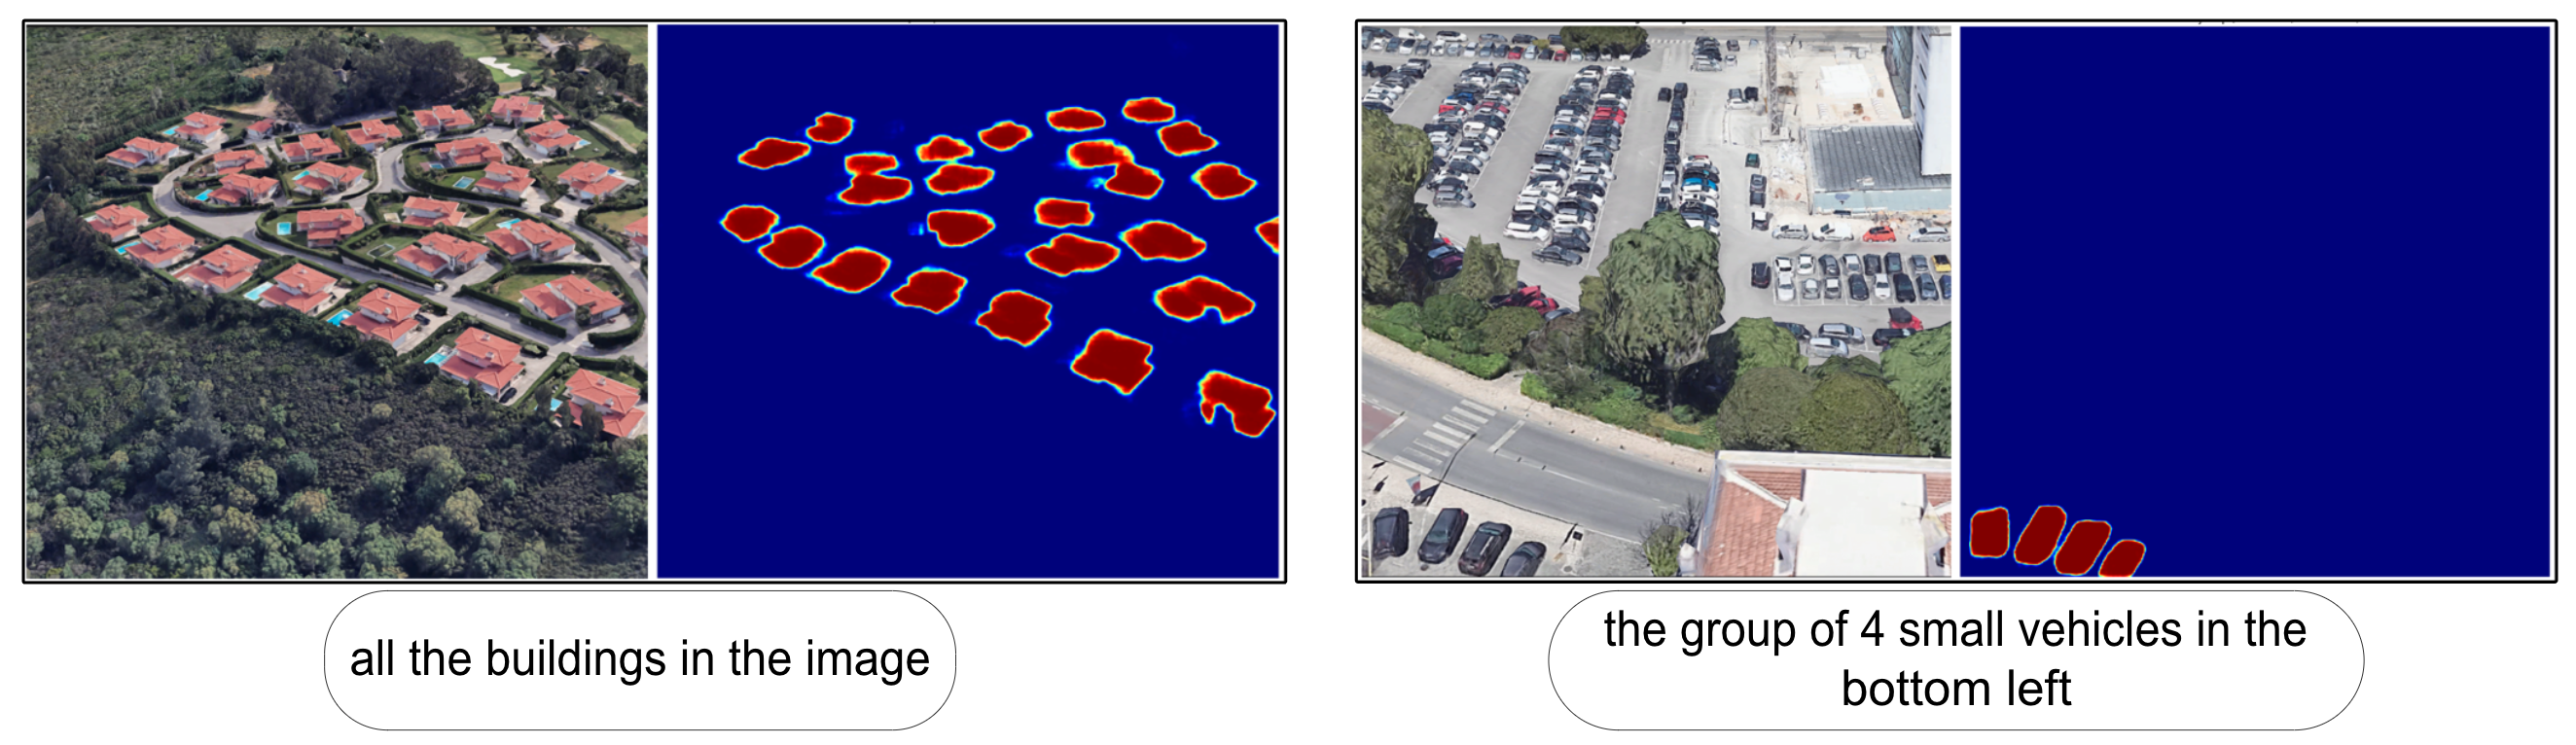
\includegraphics[width=\textwidth]{./Images/qualitative.png}
\caption{Qualitative segmentation results from RSRefSeg model on AERIAL-D validation set.}
\label{fig:qualitative_examples}
\end{figure}

The qualitative results show successful segmentation across various object categories including vehicles, buildings, water bodies, and infrastructure elements with varying spatial relationships and contextual descriptions.

\subsection{Ablation Studies}

% Ablation expression types table
\begin{table}[H]
\centering
\caption{Ablation Study: Expression Type Training Analysis}
\label{tab:ablation_expression_types}
\resizebox{\textwidth}{!}{%
\begin{tabular}{@{}lcccccc@{}}
\toprule
\textbf{Training Configuration} & \textbf{IoU@0.5} & \textbf{IoU@0.7} & \textbf{IoU@0.9} & \textbf{mIoU} & \textbf{oIoU} & \textbf{Training Expressions} \\
\midrule
Rule-based Only & -- & -- & -- & -- & -- & -- \\
Language Variations & -- & -- & -- & -- & -- & -- \\
Unique Expressions & -- & -- & -- & -- & -- & -- \\
Combined All & -- & -- & -- & -- & -- & -- \\
\bottomrule
\end{tabular}%
}
\end{table}

% #############################################################################
\section{Analysis and Discussion}
The experimental results demonstrate several key findings about open-vocabulary aerial image segmentation using the AerialD dataset:

\textbf{Dataset Scale Impact}: The significant increase in dataset size (1.5M vs. 50K expressions) enables better model generalization across diverse aerial imagery contexts and expression types.

\textbf{LLM Enhancement Benefits}: The integration of LLM-enhanced expressions improves model performance by providing more natural language variations and detailed visual descriptions that better capture real-world referring patterns.

\textbf{Multi-object Capability}: Unlike previous datasets that focus primarily on single-object referring, our approach successfully handles complex multi-object scenarios with spatial relationships and group references.

\textbf{Cross-domain Generalization}: The combination of multiple source datasets (iSAID, LoveDA, DeepGlobe) enables robust performance across different aerial imagery domains and object categories.